\section{All You Need is Combinatorics  }
In this problem, you are given an \textit{Artificial Machine(!)} and you are asked to teach it in a way
that in the end, it would Learn \textit{Intelligence(?)}. So basically, by solving this problem completely,
you will know everything needed in this course.
\subsection{A simple Random Walk}
First, suppose that our Machine shows an integer at each time and it starts with 0 at the first
round. On each round after that, the Machine randomly and with equal probability, either
increases its number by 1 or decrease it by 1 (it can show negative integers too). Calculate the
probability of our Machine showing 0 on its monitor again, if we know that it will work for
exactly $T$ rounds. (There is no need for your answer to have a closed and simple form and just
the solution is important for this part)
\begin{qsolve}
	\begin{qsolve}[]
		We employ the concept of the Khayyam-Pascal triangle to address this problem. this triangle is shown in the figure below.
		\begin{figure}[H]
			\centering
			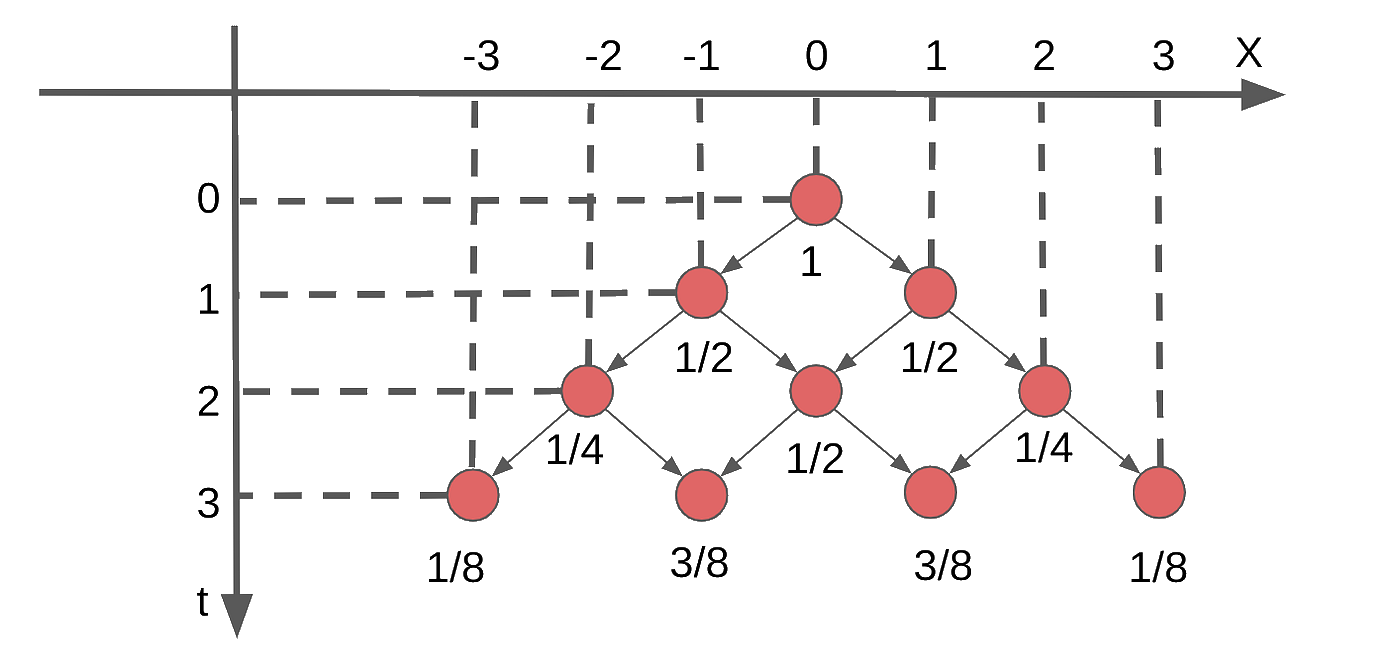
\includegraphics[width=0.5\textwidth]{khayyam_pascal_triangle.png}
			\caption{Khayyam-Pascal triangle}
		\end{figure}

		 For each time step $T$, if $T$ is odd, the probability of obtaining zero at that time step is $0$. However, if $T$ is even and we desire the result to be $0$, the counts of 1’s and -1’s must be equal. Hence, the number of instances where our machine displays 0 on its monitor again is $\binom{T}{\frac{T}{2}}$. This suggests that the number of cases is \hl{$\dfrac{T!}{\frac{T}{2}!\frac{T}{2}!}$}. The total number of possible cases is $\Sigma_{i=0}^T \binom{T}{i} = 2^T$, so the probability of our machine displaying 0 on its monitor is \hl{$\dfrac{T!}{\frac{T}{2}!\frac{T}{2}!2^T}$}.
	\splitqsolve[\splitqsolve]
	
	
		The key trick here is that if we want to compute the probability of having 0 \textbf{until} the time step $T$, we should not expand nodes of 0 in previous rows of the triangle. This is because in this case we count a stream like $[-1,1,-1,1]$ as one successful case and not two. So, at each time step, we first calculate all successful cases, then we subtract the cases that arise from expanding nodes of 0 in previous rows of the triangle. We also note that for odd $T$, the number of successful cases is the same as the number of successful cases in $T-1$. 
		
		First, we define a function called $N(T)$. This function takes the time step as input and outputs the number of successful cases (subtracting the cases that arise from expanding nodes of 0 in previous rows of the triangle). Then, the probability of having $0$ until that time step is $\dfrac{N(T)}{2^T}$. To find the total number of successful cases, we use the formula mentioned earlier. For subtraction, we utilize the fact that the number of successful cases that arise from expanding nodes of 0 in previous rows (for example, $T_1$) of the triangle equals $N(T_1)\binom{T-T_1}{\frac{T-T_1}{2}}$. This is because we can choose the number of 1's and -1's in the remaining time steps in $\binom{T-T_1}{\frac{T-T_1}{2}}$ ways and the number of successful cases in $T_1$ is $N(T_1)$. Finally, we add the probabilities of all even $T$'s until time step $T$ to find the probability. 
	

		Now, we can calculate the number of successful cases in $T$ using this formula: \textit{(X is the random variable representing the number of times the machine shows 0 on its monitor until time step T)}
				\[N(2) = 2 \Rightarrow \ P(X = 0|T = 2) = \dfrac{2}{4} = \dfrac{1}{2}\]
				\[N(4) = \binom{4}{2} - N(2)\binom{2}{1} = 6 - 4 = 2 \Rightarrow \ P(X = 0|T = 4) = \dfrac{2}{16} + \dfrac{1}{2} = \dfrac{5}{8}\]
				$$N(6) = \binom{6}{3} - N(2)\binom{4}{2} - N(4)\binom{2}{1} = 20 - 12 - 4 = 4$$
				$$\Rightarrow \ P(X = 0|T = 6) = \dfrac{4}{64} + \dfrac{5}{8} = \dfrac{11}{16}$$
				$$N(8) = \binom{8}{4} - N(2)\binom{6}{3} - N(4)\binom{4}{2} - N(6)\binom{2}{1} = 70 - 40 - 12 - 8 = 10$$ 
				$$ \Rightarrow \ P(X = 0|T = 8) = \dfrac{10}{256} + \dfrac{11}{16} = \dfrac{93}{128}$$
	\end{qsolve}
	now we use another way to get a closed form. \textbf{this proof is inspired by proof on \href{https://en.wikipedia.org/wiki/Catalan_number}{catalan numbers}}.
	\begin{qsolve}[]
		if we define a random walk of length $N$ as a sequence $w = \{\varepsilon _n\}_{n = 1}^{N} $ elementary steps $\varepsilon \in \{+1 , -1\}$ such that $S_n(w) = \sum_{i=1}^n \varepsilon _i$ and $S_0 = 0$ we can introduce the following terminology for certain special types of walks:
		\splitqsolve[\splitqsolve]
		\begin{itemize}
			\item \textbf{Balanced walk}: A walk of length $2N$ such that $S_N(w) = 0$. \textit{it contains the same number of up-steps as down-steps}
			\item \textbf{non-negetive walk}: if $S_n(w) \geq 0$ for $1\leq n \leq N$. \textit{it never goes below the initial position}
			\item \textbf{non-zero walk}: if $S_n(w) \neq 0$ for $1\leq n \leq N$. \textit{it never returns to the initial position A non-zero walk is either positive or negative depending on whether $S_n(w) > 0$ or $S_n(w) < 0$ for all $n > 1$}
		\end{itemize}
		if we define $A_n = \binom{2n}{n}$ we can proof that this is the number of :
		\begin{itemize}
			\item balanced walks of length $2n$
			\item non-negative walks of length $2n$
			\item non-zero walks of length $2n$
		\end{itemize}
		we proved that the number of balanced walks of length $2n$ is $A_n$ in previous section. for non-negetive walk of length $2n$ we can proof that the number of this kind of walks with $m$ up-steps and $k$ down-steps where $k\leq m$ is:
		$$B(m,k) = \binom{m + k}{k} - \binom{m + k}{k-1} $$
		now we can easily count all non-negetive walks of length 2n obtaining:
		$$1 + \sum _{k=1}^{n} B(2n-k,k) = 1 +  \sum _{k=1}^{n} \binom{2n}{k} - \binom{2n}{k-1} =$$
		$$ 1 + \binom{2n}{1} - \binom{2n}{0} + \binom{2n}{2} - \binom{2n}{1} + \dots + \binom{2n}{n} - \binom{2n}{n-1} = \binom{2n}{n} = A_n$$
		Hence the number of non-negetive walks of length $2n$ is also $A_n$. Furthermore, the number of positive walks of length $2n$ is the same as the number of non-negetive walks of length $2n-1$ wich is:
		$$1 + \sum _{k=1}^{n-1} B(2n-1-k,k) = \binom{2n-1}{n} = \frac{1}{2} A_n$$
		by symmetry the number of negative walks of length $2n$ is also $\frac{1}{2} A_n$. so the number of non-zero walks of length $2n$ is $A_n$. so the probability of not crossing zero in a random walk of length $2n$ is $\dfrac{A_n}{2^2n}$. in our problem we can state that the number of non crossing zero walks of length $T$ is $$P(X\neq 0|T=T) = \dfrac{\binom{T}{\lfloor \frac{T}{2} \rfloor}}{2^T}$$
		so the probability of crossing zero (wich is the answer to our question) is:
		\begin{center}
			\hl{$P(X=0|T=T) = 1 - \dfrac{\binom{T}{\lfloor \frac{T}{2} \rfloor}}{2^T}$}
		\end{center}
	\end{qsolve}

\end{qsolve}


\subsection{ Everything is possible!}
According to the previous part, show that if $T$ goes to $\infty$, then the probability of seeing 0 again
will converge to 1. Also with a similar reasoning show that we will see every other number at
least once too(for this, no calculations is needed).
\begin{qsolve}
	fo this question we use stirling's approximation. this approximation states that:
	\begin{qsolve}[]
		\begin{center}
			stirling's approximation: 
		\end{center}
		for large $n$:
		$$n! \approx \sqrt{2\pi n}\left(\dfrac{n}{e}\right)^n$$
	\end{qsolve}
	in the previous part we showed that the probability of seeing 0 again after $T$ steps is:
	$$P(X=0|T=T) = 1 - \dfrac{\binom{T}{ \frac{T}{2} }}{2^T}$$
	so we have:
	\begin{qsolve}[]
		$$P(X=0|T=T) = 1 - \dfrac{T!}{\frac{T}{2}!\frac{T}{2}! 2^T}$$
		$$\Rightarrow \lim_{T \to \infty} P(X=0|T=T) = 1 - \dfrac{\sqrt{2\pi T}\left(\dfrac{T}{e}\right)^T}{(\sqrt{2\pi \frac{T}{2}}\left(\dfrac{T}{2e}\right)^{\frac{T}{2}})^2 2^T }$$
		$$\Rightarrow \lim_{T \to \infty} P(X=0|T=T) = 1 - \dfrac{\sqrt{2\pi T}\left(\dfrac{T}{e}\right)^T}{\pi T \left(\dfrac{T}{2e}\right)^T 2^T}$$
		$$\Rightarrow \lim_{T \to \infty} P(X=0|T=T) = 1 - \dfrac{\sqrt{2\pi T}\left(\dfrac{T}{e}\right)^T}{\pi T \left(\dfrac{T}{e}\right)^T}$$
		$$\Rightarrow \lim_{T \to \infty} P(X=0|T=T) = 1 - \dfrac{\sqrt{2\pi T}}{\pi T}$$
		$$\Rightarrow \lim_{T \to \infty} P(X=0|T=T) = 1$$
		we can use a similar reasoning to show that the probability of seeing every other number at least once is 1.
		this is because the number of times we cross a number is $\binom{T}{\frac{T+k}{2}}$ \textit{for each ($k \leq T$)} and the probability of crossing a number is:
		\splitqsolve[\splitqsolve]
		$$P(X=k|T=T) = 1 - \dfrac{\binom{T}{ \frac{T+k}{2} }}{2^T}$$
		so like the proof for 0 we can show that the probability of crossing a number converges to 1 as $T$ goes to $\infty$.
	\end{qsolve}


\end{qsolve}
\subsection{ A naive algorithm}
Now, we want to teach the first Learning algorithm to our Machine. For this, suppose that we
have n secrets which are either 0 or 1 with equal probability. In other words, our whole secret
is a random vector of 0 and 1’s in $\{0, 1\}^n$, which the Machine isn’t aware of. At each round,
Machine guesses a random vector of the same form totally random(with same probability for
each vector), and it will stop whenever its guess completely match the secret. Calculate the
expected time of success for our algorithm and based on that, explain why in practice, using
such an algorithm isn’t helpful at all.
\begin{qsolve}
	\begin{qsolve}[]
		if we have a random vector of $0$ and $1$'s of length $n$ and our algorithm guesses a random vector of the same form at each round, the probability of success at each round is $\dfrac{1}{2^n}$.we can model this as a geometric distribution with parameter $p = \dfrac{1}{2^n}$. the expected number of trials until the first success is $\dfrac{1}{p} = 2^n$. so the expected time of success for our algorithm is $2^n$. as n grows, the expected time of success grows exponentially. so in practice, using such an algorithm isn’t helpful at all.
	\end{qsolve}
\end{qsolve}
\subsection{A less naive algorithm}
Now, suppose that our hidden secret is a Random Permutation of 1, 2, . . . , n. At each round,
Machine guesses the first unrevealed position of this permutation and when it guess becomes
true, it will move to the next position. Algorithm will end whenever Machine guesses all of
the secret. The algorithm which Machine makes guess at each round is as follows: for each
position of permutation, Machine start guessing from the least unrevealed number, and after
each wrong guess, guesses the next least unrevealed number. Prove that this algorithm has the
best performance, in the means of expected number of time for success. Also, calculate the
expected number of times this Machine will guess before success.
\begin{qsolve}
	\begin{qsolve}[]
		we suppose that the random variables $X_1 , X_2 , \dots X_n$ represents the number of times the Machine will guess number of an array before success. we also suppose that the random variable $S$ represents the number of times the Machine will guess before success. we can state that:
		\splitqsolve[\splitqsolve]
		$$S = \sum_{i=1}^{n} X_i$$
		now we need to calculate $E[X_i]$ for each $i$. we can state that the probability of success at each round is $\dfrac{1}{n-i+1}$. we define $E_{ij}$ as the expected value of tries for $X_i$ when we had $j$ tries before. we can state that:
		$$E_{ij} = \dfrac{1}{n-i+1} + \dfrac{n-i+1-j}{n-i+2-j}(E_{i,j+1}+1)$$
		by calculating this recursive function can say that $E[X_i] = \dfrac{n-i}{2}+1$ so now we have:
		$$E[S] = \sum_{i=1}^{n} E[X_i] = \sum_{i=1}^{n} \dfrac{n-i}{2}+1 = \dfrac{n(n+3)}{4}$$
	\end{qsolve}
\end{qsolve}
\subsection{ Gaussians everywhere}
In this part, assume that our secret is a random vector from Normal, n-dimensional distribution.
It means that each of it’s entries are from Normal distribution(Gaussian with Mean 0 and
Variance 1). Now, our algorithm is upgraded so much and it works like this: It starts from
an arbitrary vector. At each round, it randomly selects an index. After that, it samples a
random number from Normal distribution like x. Then it either adds or removes x from the
selected index, and it chooses the one which is closer to the secret in that index(assume that
somehow we can know which one is closer). The algorithm will stop whenever at each index,
difference between algorithm’s number and secret, is less than some fixed t. First show that
the best starting point for the algorithm is 0
n vector, then calculate the expected finishing time
of algorithm(there is no need to explicit calculation for the expected time and only a sketch of
the proof suffices).
\begin{qsolve}
	\begin{qsolve}[]
		first we assume that for each index $i$ the random variable $X_i$ represents the number of times the Machine will guess number of an array before success. if the first value of our algorithm is $b$ we can model this as the gaussian distribution of our samples is shifted by $t$ so it would be $\mathcal{N}(b,1)$. we want our end point to be within the range of $t$ from the secret so we can state that the probability of success at each round is $P(secret[i] - t \leq X_i \leq secret[i] + t) =$
		$$\int_{secret[i] - t}^{secret[i] + t} \dfrac{1}{\sqrt{2\pi}}e^{-\dfrac{(x-b)^2}{2}}dx$$
		if we fix all parameters except $b$ and we want to maximize this probability we can differentiate this probability with respect to $b$ and set it to zero. so we have:
		\splitqsolve[\splitqsolve]
		$$\dfrac{d}{db} \int_{secret[i] - t}^{secret[i] + t} \dfrac{1}{\sqrt{2\pi}}e^{-\dfrac{(x-b)^2}{2}}dx = 0$$
		$$\Rightarrow \int_{secret[i] - t}^{secret[i] + t} \dfrac{1}{\sqrt{2\pi}}\dfrac{2(x-b)}{2\sigma^2}e^{-\dfrac{(x-b)^2}{2}}dx = 0$$
		and this is true if $b = 0$. so the best starting point for the algorithm is the 0 vector. 

	\end{qsolve}
\end{qsolve}




